\section{Security Testing (Part 1)}

\subsection{Security Testing Methods}
{
\textbf{Purpose:} Identify, assess, and improve security posture

\textbf{Methods:}
\begin{itemize}[noitemsep]
  \item \textbf{Vulnerability Scanning} – Automated tools for known vulns (e.g., OpenVAS, LGTM)
  \item \textbf{Penetration Testing} – Manual \& tool-assisted attack simulation to find \& prove risks
  \item \textbf{Red Teaming} – Simulate real attackers to test detection/response across all layers
  \item \textbf{Purple Teaming} – Red \& Blue collaboration to improve detection \& response
  \item \textbf{Breach \& Attack Simulation (BAS)} – Automated, scripted attack scenarios (e.g., MITRE ATT\&CK)
  \item \textbf{Bug Bounty} – Crowdsourced testing (public/private), pay-per-find
\end{itemize}

\textbf{Comparison:}  
\begin{itemize}[noitemsep]
  \item \textbf{Scanning:} Known vulns in 3rd-party apps/infrastructure
  \item \textbf{Pentesting:} Custom/web apps, focused scope
  \item \textbf{Red Team:} Test defenses (SOC), full attack paths
  \item \textbf{Purple/BAS:} Improve detection, develop new rules
  \item \textbf{Bug Bounty:} Live targets, continuous findings, public feedback
\end{itemize}
}

\subsection{Penetration Testing}
{
\textbf{Definition:}
\begin{itemize}[noitemsep]
  \item Simulated attack to discover exploitable vulnerabilities and evaluate risk
  \item NIST: Mimic real-world attacks to bypass security mechanisms
\end{itemize}

\textbf{Motivations:}
\begin{itemize}[noitemsep]
  \item Uncover weaknesses missed by automated tools
  \item Validate defense mechanisms \& configurations
  \item Raise awareness, justify security budgets
  \item Fulfill compliance (e.g., PCI-DSS, HIPAA)
\end{itemize}

\textbf{Scope Targets:}
\begin{itemize}[noitemsep]
  \item IT Assets – Web apps, networks, infrastructure
  \item Data – Customer info, credentials
  \item Physical – Building entry
  \item Social – Phishing, manipulation
\end{itemize}

\textbf{Success Factors:} Skills, creativity, tools, lateral thinking
}

\subsection{Penetration Testing Methodologies}
{
\begin{itemize}[noitemsep]
  \item \textbf{OSSTMM} – Full-spectrum testing, formalized scoring model
  \item \textbf{OWASP Testing Guide} – Web app testing procedures \& tools
  \item \textbf{NIST SP 800-115} – General framework, tools, validation
  \item \textbf{PTES} – Practical industry guide (incomplete/outdated)
\end{itemize}

Other resources: SANS checklists, training materials
}

\subsection{Pentest Phases}
{
\begin{enumerate}[noitemsep]
  \item \textbf{Pre-engagement} – Define scope, methods, rules, contacts
  \item \textbf{Intelligence Gathering} – Collect public/recon info
  \item \textbf{Threat Modeling} – Map potential attack paths
  \item \textbf{Vulnerability Analysis} – Identify exploitable issues
  \item \textbf{Exploitation} – Gain access or demonstrate impact
  \item \textbf{Post-Exploitation} – Lateral movement, persistence
  \item \textbf{Reporting} – Document findings, risk, mitigation
\end{enumerate}
}

\subsection{Pre-Engagement Phase}
{
\textbf{Scope:}
\begin{itemize}[noitemsep]
  \item What systems, techniques, and depth of testing
  \item Channels: physical, human, network, wireless, telecom
  \item Define inclusions/exclusions (e.g., "all except billing module")
\end{itemize}

\textbf{Rules of Engagement:}
\begin{itemize}[noitemsep]
  \item Test windows (e.g., 20:00–06:00), backup constraints
  \item Use of stealth/evasion (depends on method: black/gray/white box)
  \item Evidence handling – encrypted, need-to-know access
  \item \textbf{Permission to Test Document} – mandatory, defines scope, 3rd party authorization, liability
\end{itemize}

\textbf{Communication:}
\begin{itemize}[noitemsep]
  \item Define secure channels (e.g., file sharing, IM, phone)
  \item Emergency contacts for incident handling
  \item Frequency of status reporting
\end{itemize}

\textbf{Pitfalls:}
\begin{itemize}[noitemsep]
  \item Clients unclear on purpose (real risk vs checkbox)
  \item Scope Creep – informal extensions must be managed properly
\end{itemize}
}

\subsection{Common Test Models (OSSTMM)}
{
\begin{itemize}[noitemsep]
  \item \textbf{Blind} – Testers get no info (like attackers)
  \item \textbf{Double Blind} – Even defenders don’t know
  \item \textbf{Gray Box} – Limited internal info shared
  \item \textbf{White Box} – Full internal info shared
  \item \textbf{Crystal Box / Tandem} – Collaboration with client
  \item \textbf{Reversal / Red Teaming} – Realistic adversary simulation
\end{itemize}
}
\begin{center}
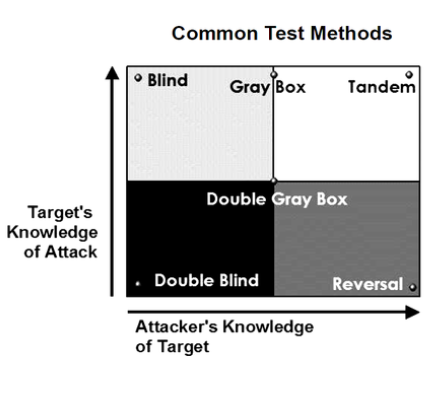
\includegraphics[width=0.75\linewidth]{Common Test Methods.png}
\end{center}

\subsection{Evidence Handling}
{
\begin{itemize}[noitemsep]
  \item Avoid storing PII/PHI unless necessary
  \item Prove access via: screenshots, permission lists, flags
  \item All data must be encrypted and access-limited
\end{itemize}
}

\subsection{Testing Method Comparison}

\subsubsection{Vulnerability Scanning}
\begin{itemize}[noitemsep]
  \item \textbf{What:} Automated scanning for known vulnerabilities using signatures
  \item \textbf{Purpose:} Identify known vulnerabilities early
  \item \textbf{Compliance:} GDPR, HIPAA, PCI-DSS
  \item \textbf{Assets:} Source code, applications, infrastructure
  \item \textbf{Result:} List of potential vulns + risk rating
  \item \textbf{Method:} Tools like OpenVAS, LGTM; fully automated
  \item \textbf{Requirement:} Vulnerability mgmt. capability (triage + patching)
  \item \textbf{Frequency:} Continuous (due to changing signatures and assets)
\end{itemize}

\subsubsection{Classical Penetration Testing}
\begin{itemize}[noitemsep]
  \item \textbf{What:} Ethical hacking to discover and verify vulnerabilities
  \item \textbf{Purpose:} Find easy-to-moderate vulns + remediation advice
  \item \textbf{Assets:} Limited scope (app, service, system)
  \item \textbf{Result:} Verified vulns, risk scores, how-to-fix
  \item \textbf{Method:} Manual + tools (OWASP Testing Guide)
  \item \textbf{Requirement:} Test environment + vuln mgmt.
  \item \textbf{Frequency:} 1–4×/year or per release cycle
\end{itemize}

\subsubsection{Red Team Testing}
\begin{itemize}[noitemsep]
  \item \textbf{What:} Realistic attack simulation to test detection/response
  \item \textbf{Purpose:} Measure SOC effectiveness and incident handling
  \item \textbf{Assets:} Broad – physical, human, cyber layers
  \item \textbf{Goal:} Achieve mission (e.g., steal data) without detection
  \item \textbf{Result:} Goal outcome + detailed attack path
  \item \textbf{Method:} Custom attack scenarios (may include social engineering)
  \item \textbf{Requirement:} Mature security org (IR, SOC, controls)
  \item \textbf{Frequency:} Periodic (e.g., annually)
\end{itemize}

\subsubsection{Purple Team Testing}
\begin{itemize}[noitemsep]
  \item \textbf{What:} Red + Blue collaboration for better detection/prevention
  \item \textbf{Purpose:} Improve SOC rules, detection logic, tuning
  \item \textbf{Assets:} Selected systems, employee targets
  \item \textbf{Result:} Improved detection rules, hardening plans
  \item \textbf{Method:} Controlled attack simulation + feedback loop
  \item \textbf{Requirement:} Cross-team collaboration
  \item \textbf{Frequency:} Periodic (e.g., quarterly)
\end{itemize}

\subsubsection{Breach \& Attack Simulation (BAS)}
\begin{itemize}[noitemsep]
  \item \textbf{What:} Continuous, automated kill chain simulation
  \item \textbf{Purpose:} Evaluate SOC resilience using known attack paths
  \item \textbf{Assets:} Based on selected attack scripts (e.g., MITRE ATT\&CK)
  \item \textbf{Result:} Summary of detection/resistance to scripted attacks
  \item \textbf{Method:} Automated platforms (SaaS)
  \item \textbf{Requirement:} Like Purple Team, but with budget for automation
  \item \textbf{Frequency:} Continuous
\end{itemize}

\subsubsection{Bug Bounty Programs}
\begin{itemize}[noitemsep]
  \item \textbf{What:} Crowdsourced vulnerability testing
  \item \textbf{Purpose:} Discover real-world vulnerabilities
  \item \textbf{Type:} Public (anyone) or Private (invite-only)
  \item \textbf{Assets:} Mostly apps/services with clear rules
  \item \textbf{Result:} Vulnerability reports with PoCs
  \item \textbf{Method:} According to platform rules (HackerOne, Bugcrowd, etc.)
  \item \textbf{Requirement:} Legal setup + risk acceptance
  \item \textbf{Frequency:} Continuous
\end{itemize}
\section{Penetration Testing (Part II)}

\subsection{Intelligence Gathering}

\textbf{Goal:} Collect relevant information from public sources to aid attacks

\textbf{Types:}
\begin{itemize}[noitemsep]
  \item Physical – maps, building layout
  \item Logical – org charts, partners
  \item Infrastructure – IPs, domains, hosts
  \item Documents – metadata, open data leaks
  \item HUMINT – staff info, social profiles
\end{itemize}

\textbf{Levels:}
\begin{itemize}[noitemsep]
  \item L1: Automated (compliance-focused)
  \item L2: Tools + manual (best-practice)
  \item L3: Manual, stealthy, social-focused (APT-style)
\end{itemize}

\textbf{Techniques:}
\begin{itemize}[noitemsep]
  \item Passive – undetectable (e.g., Shodan, WHOIS)
  \item Semi-passive – DNS queries, public info
  \item Active – detectable (e.g., scanning)
\end{itemize}

\subsection{Recon Techniques \& Tools}

\textbf{Website Analysis:} Org data, staff, emails

\textbf{Google Dorking:}
\begin{itemize}[noitemsep]
  \item Operators: \texttt{inurl:}, \texttt{intitle:}, \texttt{ext:}
  \item Tools: GHDB, ExploitDB
\end{itemize}

\textbf{Domain/IP Discovery:}
\begin{itemize}[noitemsep]
  \item WHOIS, SAN certs, Robtex, FindSubdomains
  \item DNS Tools: \texttt{dig}, \texttt{nslookup}
  \item RIR lookup, BGP Toolkit
\end{itemize}

\textbf{Passive Tools:} Shodan, Censys, Maltego

\subsection{Scanning}

\textbf{Purpose:} Map attack surface – find hosts, ports, services

\textbf{Nmap:}
\begin{itemize}[noitemsep]
  \item \texttt{-sS}: SYN scan (stealth)
  \item \texttt{-sT}: TCP connect
  \item \texttt{-sU}: UDP scan
  \item \texttt{-sV}, \texttt{-O}, \texttt{-A}, \texttt{-p-}
  \item NSE scripts: \texttt{--script=banner}, etc.
\end{itemize}

\textbf{Network Tools:} \texttt{traceroute}, \texttt{hping3}, \texttt{telnet}, \texttt{nc}, \texttt{openssl}

\subsection{Footprinting Defenses \& HUMINT}

\textbf{Identify:} Firewalls, WAFs, IDS
\begin{itemize}[noitemsep]
  \item Tools: Nmap scripts, banner fingerprinting
  \item Techniques: Packet crafting, evasion, SE
\end{itemize}

\textbf{Human Intelligence:}
\begin{itemize}[noitemsep]
  \item Social media analysis, username lookup (Knowem, etc.)
  \item Pretexting, phishing, physical visits
\end{itemize}

\section{Penetration Testing (Part III)}
\subsection{Threat Modeling}
{
\textbf{Purpose:} Identify vulnerabilities by analyzing system designs and attacker goals.

\begin{itemize}[noitemsep]
  \item \textbf{Attacker-Centric:} Map how attackers move from entry points to target assets.
  \item \textbf{Defender-Centric:} Map organizational defenses and simulate attack paths avoiding them.
  \item \textbf{Techniques:} STRIDE, Attack Trees
  \item \textbf{Assets:}
    \begin{itemize}
      \item Primary: Within test scope (e.g., CRM frontend)
      \item Secondary: Outside scope but shared (e.g., employee DB on same server)
    \end{itemize}
  \item \textbf{Threat Relevance:} Secondary assets may alter attacker models (e.g., insiders become relevant).
\end{itemize}
}
\subsection{Attack Patterns and Frameworks}{
\begin{itemize}[noitemsep]
  \item \textbf{CAPEC:} Focused on application-level attacks and training
  \item \textbf{MITRE ATT\&CK:} Real-world adversarial behavior, red-team and defense-oriented
  \item CAPEC and ATT\&CK are complementary and cross-referenced
\end{itemize}
}
\subsection{Vulnerability Analysis}
{
\textbf{Goal:} Discover and confirm security issues that can be exploited.

\textbf{Techniques:}
\begin{itemize}[noitemsep]
  \item Scanners: Nmap, Nessus, GVM, sqlmap, XSStrike
  \item Source code scanners, manual analysis (e.g., CIS Benchmarks)
  \item Web scanners: Crawl and test input points
  \item Active fuzzing: E.g., American Fuzzy Lop
  \item Track findings with attack trees to avoid redundant work
\end{itemize}

\textbf{Challenges:}
\begin{itemize}[noitemsep]
  \item \textbf{False Positives:} Patched systems not reflected in version info
  \item \textbf{False Negatives:} Backported fixes not updating version number
  \item \textbf{Environment Dependent:} Network position, authentication, etc.
\end{itemize}
}
\subsection{Exploitation}
{
\textbf{Goal:} Gain access by leveraging vulnerabilities.

\textbf{Methods:}
\begin{itemize}[noitemsep]
  \item Exploits: SQL injection, buffer overflows, MitM, USB, social engineering
  \item Select vector based on success/detection probability
  \item Consider mitigation bypass: DEP, ASLR, AV, WAF
\end{itemize}

\textbf{Expertise Levels:}
\begin{itemize}[noitemsep]
  \item \textbf{Basic:} Use public exploits
  \item \textbf{Advanced:} Modify/tune exploits and payloads
  \item \textbf{Expert:} Discover new vulnerabilities (zero-days), reverse engineering
\end{itemize}
}
\subsection{Post Exploitation}{
\textbf{Goal:} Assess value of access and maintain control (e.g., lateral movement).

\textbf{Activities:}
\begin{itemize}[noitemsep]
  \item Pivoting, island hopping
  \item Follow rules of engagement to prevent real harm
\end{itemize}
}
\subsection{Metasploit Framework (MSF)}{
\textbf{Purpose:} Exploit development and execution platform.

\textbf{Modules:}
\begin{itemize}[noitemsep]
  \item \textbf{Exploits:} Execute payloads
  \item \textbf{Payloads:} Single (self-contained), stagers/stages (modular)
  \item \textbf{Meterpreter:} Advanced in-memory post-exploitation agent
  \item \textbf{Auxiliary:} Scanning, info gathering, DoS
  \item \textbf{Post:} System interaction, enumeration, credential dumping
\end{itemize}

\textbf{Architecture:}
\begin{itemize}[noitemsep]
  \item Ruby-based, modular structure
  \item msfconsole: Primary CLI interface
  \item Can integrate with external tools (Nmap, Nessus)
\end{itemize}
}
\subsection{Lab: Exploitation and Metasploit}
{
\textbf{Goal:} Learn practical exploitation using the Metasploit Framework (MSF).

\textbf{Target Environment:}
\begin{itemize}[noitemsep]
  \item Vulnerable Linux machine in virtual lab setup
  \item Services exposed: SSH, Samba, HTTP
\end{itemize}

\textbf{Key Commands:}
\begin{itemize}[noitemsep]
  \item \texttt{nmap -sS -sV -O -A <IP>} – scan target for open ports and services
  \item \texttt{msfconsole} – launch Metasploit CLI
  \item \texttt{search <keyword>} – find exploits or modules
  \item \texttt{use <module>} – load exploit/module
  \item \texttt{set RHOST <IP>} – set remote host
  \item \texttt{set PAYLOAD <payload>} – select appropriate payload
  \item \texttt{exploit} – execute attack
  \item \texttt{sessions -i <id>} – interact with session
  \item \texttt{getuid}, \texttt{sysinfo}, \texttt{ps}, \texttt{hashdump}, \texttt{shell} – post-exploitation
\end{itemize}

\textbf{Exploitation Process:}
\begin{itemize}[noitemsep]
  \item Scan for vulnerable services (e.g., VSFTPD)
  \item Search and select matching exploit in Metasploit
  \item Configure exploit parameters (RHOST, RPORT, payload)
  \item Launch exploit and gain reverse shell via Meterpreter
\end{itemize}

\textbf{Metasploit Modules Used:}
\begin{itemize}[noitemsep]
  \item \textbf{Exploit:} \texttt{exploit/unix/ftp/vsftpd\_234\_backdoor}
  \item \textbf{Payload:} \texttt{linux/x86/meterpreter/reverse\_tcp}
  \item \textbf{Auxiliary:} \texttt{scanner/portscan/tcp}, \texttt{scanner/ftp/ftp\_version}
\end{itemize}

\textbf{Post-Exploitation Tasks:}
\begin{itemize}[noitemsep]
  \item Enumerate users/processes
  \item Dump password hashes (\texttt{hashdump})
  \item Launch interactive shell or pivot to further targets
\end{itemize}

\textbf{Key Learnings:}
\begin{itemize}[noitemsep]
  \item How to map vulnerabilities to working exploits
  \item Effective use of Meterpreter for post-exploitation
  \item Importance of version info and accurate scanning
\end{itemize}
}
